\def\latexktupreamblefile{scoring_manual.ktu_preamble}
\def\mytitle{scoringパッケージ}
\def\myauthor{山本}
\def\mydate{2019.6.25}
\def\latexxspacing{no}
\input{ltktu.tex}

\newcommand {\mycolor }{olive}

\section{scoringパッケージの概要}
\label{scoringパッケージの概要}

(この\texttt{readme.md}をtexでpdfにしたファイルが\texttt{manual\slash scoring\_manual.pdf}にある)

採点作業の流れの中で以下のような作業をscoringパッケージはサポートする。

\begin{enumerate}
\item マークシートの採点

\begin{itemize}
\item マークシートの読取結果(csvファイル)を採点し、学籍番号と点数のcsvファイルを作成する

\end{itemize}

\item 統合

\begin{itemize}
\item マークシート以外の成績情報を統合する(例えば、宿題や筆記問題の採点結果などとの統合)

\end{itemize}

\item 分析

\begin{itemize}
\item 以下のような統計データを出力できるので、それを見て分析する

\item 各問題の正解割合, 評語(A+ABCD)の割合, 点数のヒストグラム, 基本統計, 学類別基本統計

\end{itemize}

\item 点数調整

\begin{itemize}
\item 点数調整を行って配点を調整する

\end{itemize}

\item Twinsへの成績アップロード用ファイルの作成

\begin{itemize}
\item 点数調整を行った最終結果をtwinsのアップロード用ファイルに統合する

\end{itemize}

\item 記録: twins名簿をベースに記録用のファイル作成

\end{enumerate}

\section{install}
\label{install}

installは以下の2つのファイルを正しい場所に配置すればよい。

\begin{itemize}
\item \texttt{src\slash scoring.py}: pythonのプログラム(モジュール)なので、pythonのライブラリパスが
通っているところにコピーする。

\item \texttt{bin\slash score}: scoringパッケージを呼び出すbashシェルなので、\texttt{PATH}が通っているところにコピーする。
scoringパッケージのすべての機能はこの\texttt{score}コマンドを通して提供される。

\end{itemize}

\texttt{make install}で配置したい場合は\texttt{Makefile}の中の以下の2つの変数を
正しくセットしてから、\texttt{make install}する。
\begin{tcolorbox}[enhanced jigsaw,breakable,colframe=\mycolor ,colback=white,colbacktitle=\mycolor ,coltitle=white,fonttitle=\bfseries\sffamily]

\begin{verbatim}
pylib = scoring.pyを入れるディレクトリ(普通は$PYTHONPATH)
bindir = scoreコマンドを入れるディレクトリ($PATHのどれか)
\end{verbatim}

\end{tcolorbox}

前提条件は以下。

\begin{itemize}
\item python3.6以上

\item pythonのpandasモジュール

\end{itemize}

\section{scoreコマンドの使い方}
\label{scoreコマンドの使い方}

scoringパッケージのすべての機能は\texttt{score}コマンドを経由して
提供される。すべての成績データ(入力・出力・途中結果)は学籍番号を必ず含む
csvファイルで表現される。\texttt{score}コマンドは少なくとも1つのcsvファイルを扱うので、
1つのcsvファイルは必須引数である。基本的に出力は\texttt{stdout}にcsvの形式で
加工された成績が出力される。また、分析用の情報は\texttt{stderr}に出力される。
\begin{tcolorbox}[enhanced jigsaw,breakable,colframe=\mycolor ,colback=white,colbacktitle=\mycolor ,coltitle=white,fonttitle=\bfseries\sffamily,title=\texttt{\$ score -h}]

\begin{verbatim}
usage: score [-h] [-marksheet ref-file desired_pscore] [-crate]
             [-twins] [-join csvfile2] [-record csvfile2 [csvfile2 ...]]
             [-adjust x y xmax] [-interval min max]
             [-distribution] [-abcd] [-statistics] [-gakuruistat csv-meibo-utf8]
             [-nostdout] [-output filename]
             csvfile
\end{verbatim}

\end{tcolorbox}

オプション名は区別が可能な限り短縮してよい。`\texttt{-adjust}'と`\texttt{-abcd}'オプション以外は
すべて1文字で区別できる。

必須引数である\texttt{csvfile}は次のように4種類に解釈される。

\begin{itemize}
\item \texttt{-marksheet}オプションが指定された場合

\begin{itemize}
\item マークシートの読取結果(学生の解答ファイル)とみなされる

\begin{itemize}
\item headerなし

\item 1列目が学籍番号(下7桁), 2列目以降はマークシートのマーク番号

\end{itemize}

\end{itemize}

\item \texttt{-twins}オプションが指定された場合

\begin{itemize}
\item twinsからダウンロードした成績アップロード用csvファイルとみなされる

\begin{itemize}
\item twinsからダウンロードしたままのファイルでOK

\item headerあり(ただし、読み込み時には無視する(sjis\&ラベルに変なスペースが入っているため))

\item 列は左から'科目番号`,'学籍番号`, `学期区分','学期評価', `総合評価'

\end{itemize}

\end{itemize}

\item \texttt{-record}オプションが指定された場合

\begin{itemize}
\item twinsからダウンロードされた名簿ファイルとみなされる

\begin{itemize}
\item twinsからダウンロードしたままのファイルでOK

\item ただし、`\texttt{csv}'と`\texttt{utf8}'を指定してダウンロードしたファイルに限る

\end{itemize}

\end{itemize}

\item 上記以外

\begin{itemize}
\item 採点途中結果のcsvファイル

\begin{itemize}
\item headerなし

\item 1列目が学籍番号(9桁), 2列目が点数

\end{itemize}

\end{itemize}

\end{itemize}
結果的に、上の3つのオプションは排他的である。

\texttt{score}コマンドの出力は`\texttt{-twins}'または`\texttt{-record}'オプションが指定された場合を除いて、
すべて「採点途中結果のcsvファイル(headerなしの1列目が学籍番号(9桁),2列目が点数)」である。

以下では、作業の種別毎にオプションを説明する。

\subsection{マークシート採点}
\label{マークシート採点}

\subsubsection{\texttt{score csvfile -marksheet ref-file desired-pscore [-crate] ...}}
\label{scorecsvfile-marksheetref-filedesired-pscore-crate...}

\texttt{csvfile}をマークシート読み取り結果ファイルとして読み込み、採点を行う。
マークシートの正解を定義したファイル(\texttt{ref-file})を引数として与える。
また、マークシートの満点(\texttt{desired-pscore})を与える。正解定義中の各問題のweightに
したがって各問題に配点する(配点は整数なので要求した満点と
少し違うこともありえる)。
\texttt{-twins}と\texttt{-record}以外の全てのオプションを同時に使用可能。
チェック用として各学生・各問題ごとの正誤(正=1, 誤=0)のcsvファイルを以下の
名称で保存する。

\begin{itemize}
\item \texttt{\$(csvfile).marubatu}

\end{itemize}

マークシート採点のための正解定義は\ref{mksheet-ref}節参照。
学籍番号はすべて頭に\texttt{20}が付けられるので(\texttt{200000000}を足す)、
必ず下7桁になっている必要がある。

\texttt{-crate}オプションは、\texttt{-marksheet}オプションが指定されているときだけ有効な
オプションで、各小問毎の正解率、配点、問題タイプを\texttt{stderr}に出力する。

\subsection{統合とtwinsアップロードファイルの作成}
\label{統合とtwinsアップロードファイルの作成}

\subsubsection{\texttt{score csvfile -join csvfile2 ...}}
\label{scorecsvfile-joincsvfile2...}

必須ファイル\texttt{csvfile}で指定されたデータ\floatfootnote{\texttt{-marksheet}オプションが指定されている場合は、採点結果に対して適用される。}に\texttt{csvfile2}で
指定されるデータを統合(点数の合算)する。統合は、keyとして学籍番号を用い、
\texttt{pandas}の\texttt{merge}関数を用いる。統合(join)方法は以下の2種類。

\begin{itemize}
\item \texttt{-twins}オプションが指定されている場合:

\begin{itemize}
\item twinsアップロードファイルへleft-joinを行う。

\begin{itemize}
\item twinsのファイルにない学生は取り除かれる

\item 取り除く学生の学籍番号はstderrに出力される

\end{itemize}

\end{itemize}

\item \texttt{-twins}オプションがない場合:

\begin{itemize}
\item outer-joinを行う

\begin{itemize}
\item 片方のデータにしかない学生も残る。

\item データがない方の学生の点数は0点

\end{itemize}

\end{itemize}

\end{itemize}

\texttt{-twins}オプションがある場合の出力はtwinsへのアップロード用の
ファイルとして出力される。

\begin{itemize}
\item headerがshift-jisでないといけないので\texttt{-output}オプションでファイルを指定する。

\begin{itemize}
\item 標準出力に出すとなぜかshift-jisにならない\frownie 

\end{itemize}

\item twinsデータの'総合評価'に数値が入っている場合はそれと\texttt{csvfile2}の点数の合計が'総合評価'になる

\item twinsデータの'総合評価'が空の場合は\texttt{csvfile2}の点数が'総合評価'になる

\end{itemize}

\texttt{-join}オプションの引数である\texttt{csvfile2}のファイルの仕様は以下。

\begin{itemize}
\item headerなし

\item 1列目: 学籍番号

\item 2列目以降(いくつでもOK): 評価点

\begin{itemize}
\item 2列目以降の点数は合計される

\item 統合後に\texttt{csvfile}と\texttt{csvfile2}の点数は合計される

\end{itemize}

\end{itemize}

他のあらゆるオプションを同時使用可能。

\subsection{点数調整}
\label{点数調整}

点数調整は、マークシート採点後または統合後、あるいはどちらも指定されてない場合は
\texttt{csvfile}で与えられた処理途中のデータに対して適用される。

\subsubsection{\texttt{score csvfile ... -adjust x y xmax}}
\label{scorecsvfile...-adjustxyxmax}

素点xをyに線型に持ち上げる。xmax以上は素点のまま。
図\ref{fig:adjust}を参照。

\begin{figure}[htbp]
\centering
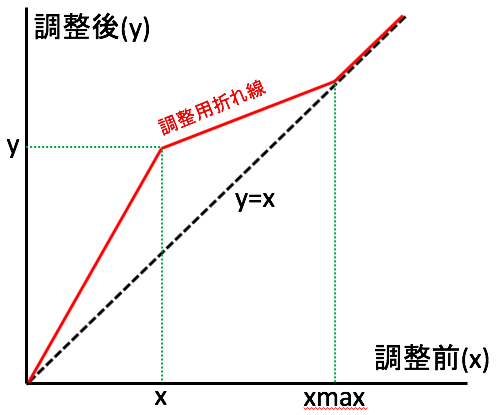
\includegraphics[keepaspectratio,width=5cm,height=0.75\textheight]{fig/adjust.png}
\caption{\texttt{-adjust x y xmax}の点数調整}
\label{fig:adjust}
\end{figure}

\subsubsection{\texttt{score csvfile ... -interval min max}}
\label{scorecsvfile...-intervalminmax}

点数の最低点を\texttt{min}、最高点を\texttt{max}にする。単に範囲からはみ出した点数を
\texttt{min}と\texttt{max}に置き換えるだけ。線型変換などはしない。

\subsection{分析}
\label{分析}

分析は点数調整後の成績に対して行われる(すなわち出力ファイルに対する
分析である)。以下のような種類(オプション名)があり、同時に指定できる。
出力はすべて\texttt{stderr}に出力される。

\begin{itemize}
\item \texttt{-distribution}: 点数分布のヒストグラム出力

\item \texttt{-abcd}: 標語(A+, A, B, C, D)の人数分布

\item \texttt{-statistics}: 平均, 標準偏差, 最高・最低点, 4分位点

\item \texttt{-gakuruistat csv-meibo-utf8}: 学類毎の\texttt{statistics}

\begin{itemize}
\item \texttt{csv-meibo-utf8}はtwinsからダウンロードした名簿ファイル

\begin{itemize}
\item csvでかつutf8を指定してダウンロード

\item (`\texttt{-record}'オプションで与える名簿と同じファイルでOK)

\end{itemize}

\end{itemize}

\end{itemize}

\texttt{-record}オプションを除くあらゆる他のオプションと同時併用できる。
最終結果(すなわち出力データ)に対する分析を行う。先に行われるのは、
マークシート採点、統合、点数調整である。
いずれも指定されていない場合は、入力としての\texttt{csvfile}がそのまま
分析対象となる。\texttt{-twins}オプションが指定されている場合は、
twinsへのアップロードファイルの分析が行われる。

点数調整と分析は同時に指定しながら調整するのが普通の使い方と思われる。

\subsection{記録}
\label{記録}

採点途中の結果を学籍番号・氏名付きのファイルにまとめて記録用のファイルを作成する
オプションが以下の\texttt{-record}である。

\begin{itemize}
\item \texttt{score csvfile -record csvfile2 [csvfile2 ...] [-output excel-filename]}

\end{itemize}

このオプションが指定されると、必須引数\texttt{csvfile}はtwinsからダウンロード
された名簿ファイルとみなされる。これは\texttt{-gakuruistat}の引数と同じファイルで、
twinsからダウンロードしたままの名簿ファイルでOK。ただし、`\texttt{csv}'と`\texttt{utf8}'を
指定してダウンロードしたファイルに限る。以下のような処理を行う。

\begin{itemize}
\item 上記の名簿にこのオプションの引数\texttt{csvfile2}(複数指定できる)をouter-joinする。

\item 点数の合算などはしない

\item \texttt{csvfile2}は必ず1列目が学籍番号でなければならない(\texttt{csvfile2}に
twinsファイルは指定できない)。その他の列は文字列でもなんでもかまわない。

\item `\texttt{-output}'オプション以外のすべてのオプションが無視される。

\item `\texttt{-output}'オプションを指定するとExcelファイルが\texttt{-output}オプションで
指定したファイル名のファイルとして出力される。

\begin{itemize}
\item この場合、\texttt{filename}の拡張子は\texttt{xlsx}がよいと思われる。

\item Headerは名簿ファイルの項目についてしか入ってないので、
出力後に各列の意味を手動で入力する必要がある。

\end{itemize}

\item `\texttt{-output}'オプションがない場合は、utf8のcsvファイルとしてstdoutに出力される。

\end{itemize}

\subsection{その他}
\label{その他}

その他のオプションは以下。

\begin{itemize}
\item \texttt{-nostderr}: 標準出力に結果のcsvファイルを出力しない

\begin{itemize}
\item 調整時にこれを指定することが多い

\end{itemize}

\item \texttt{-output filename}: 結果を標準出力ではなくファイルに出力する

\begin{itemize}
\item twinsアップロード用ファイルはこのオプションで出力しないと
headerが正しくshift-jisで出力されない

\item `\texttt{-record}'オプションが指定されている場合は、Excelファイルが出力される。

\end{itemize}

\end{itemize}

\section{使用例}
\label{使用例}

\subsection{使用例1}
\label{使用例1}

ある科目の使用例。この科目では期末試験でマークシート問題と記述問題の
2種類の解答をしてもらった。また、宿題の点数が別に定義されている。

\begin{enumerate}
\item ファイルの準備

\begin{itemize}
\item answer.csv: マークシートの読み取り結果

\item sup.csv: 記述問題の採点結果と宿題の点数(1列目が学籍番号, 2列目と3列目にそれぞれの点数)

\item upload.csv: twinsからダウンロードした成績アップロード用ファイル

\begin{itemize}
\item ファイル形式の指定はできない(csvでshift-jis) (そのままでよい)

\end{itemize}

\item meibo.csv: twinsからダウンロードした名簿ファイル

\begin{itemize}
\item csvかつutf8を指定してダウンロード

\end{itemize}

\item refrence.py: マークシートの正解と配点重みを定義したファイル

\begin{itemize}
\item pythonのlist形式の記述なので拡張子を\texttt{py}としているが、
気持ち悪ければ\texttt{txt}でもOK

\end{itemize}

\end{itemize}

\item マークシートの採点

\begin{itemize}
\item 小問の正解率と満点を80としたときの配点等の情報を保存

\begin{itemize}
\item \$ score answer.csv -m reference.py 80 -c -n \&> crate.txt

\end{itemize}

\item マークシートだけの得点状況を分析

\begin{itemize}
\item \$ score answer.csv -m reference.py 80 -s -d -abcd -n

\item 分析結果を残したい場合は最後に\texttt{\&> file.txt}を付ける

\item この結果から正解の配点重みを変更してもよい

\end{itemize}

\item (マークシートだけの得点を少し調整する場合)

\begin{itemize}
\item \$ score answer.csv -m reference.py 80 -d -adjust x y xmax -n

\end{itemize}

\item 採点結果を書き出す

\begin{itemize}
\item \$ score answer.csv -m reference.py 80 {[-adjust x y xmax]} > mksheet.csv

\end{itemize}

\end{itemize}

\item マークシート以外の点数を統合

\begin{itemize}
\item sup.csvを統合する

\begin{itemize}
\item \$ score mksheet.csv -j sup.csv > mksheet\_sup.csv

\end{itemize}

\end{itemize}

\item 得点調整を行う

\begin{itemize}
\item 例えば、\texttt{-adjust}オプションを使って調整する

\begin{itemize}
\item \$ score mksheet\_sup.csv -abcd -d -adjust x y xmax -n

\item (最低・最高点が{[0,100]}をはみ出す場合は\texttt{-i 0 100}を加える)

\end{itemize}

\item 結果を書き出す

\begin{itemize}
\item \$ score mksheet\_sup.csv -abcd -d -adjust x y xmax > mksheet\_sup\_adjust.csv

\end{itemize}

\item (上記の2つの手順は同時に行うこともできる)

\begin{itemize}
\item \$ score mksheet.csv -j sup.csv -abcd -d -adjust x y xmax > mksheet\_sup\_adjust.csv

\end{itemize}

\end{itemize}

\item twinsのアップロードファイルを作成

\begin{itemize}
\item \$ score upload.csv -t -j mksheet\_sup\_adjust.csv -d > twins\_upload.csv

\item (最低・最高点が{[0,100]}をはみ出す場合は\texttt{-i 0 100}を加える)

\end{itemize}

\item 特別処理が必要な学生に対してtwins\_upload.csvを直接修正

\item 最終結果に対する分析結果を保存

\begin{itemize}
\item \$ score twins\_upload.csv -t -s -g meibo.csv -d -abcd -n \&> result\_analysis.txt

\end{itemize}

\item 氏名、学籍番号と採点途中結果を履歴として残す

\begin{itemize}
\item \$ score meibo.csv -record mksheet.csv sup.csv mksheet\_sup.csv mksheet\_sup\_adjust.csv -o matome.xlsx

\item \texttt{matome.xlsx}に手作業でラベルなどを付ける

\end{itemize}

\end{enumerate}

\subsection{使用例2}
\label{使用例2}

\texttt{test}ディレクトリ以下に簡単なデータが準備してある。
準備されているデータは例として参考にしてください。
\texttt{test}ディクレトリで\texttt{auto.sh}を起動すると使用例1の簡単化された手続きが実行される。
結果の例が\texttt{test\slash test-ref}ディレクトリ以下にあるので正しく動作しているかを確認のためにも使える。

\section{付録}
\label{付録}

\subsection{準備作業}
\label{準備作業}

必要な準備作業を以下にまとめる。

\subsubsection{マークシート読み取り}
\label{マークシート読み取り}

学類所有のマークシート読み取り装置を使って読み取る。
前提としているマークシートは以下。

\begin{itemize}
\item 教育ソフトウェア社の「総合カード053」(型番: C053)

\begin{itemize}
\item 学生番号欄: 7桁(なので、学籍番号下7桁をマークさせる)

\item 解答欄: 「1--9,0」の0--9の数をマークできる列が50列

\begin{itemize}
\item 上から1,2,3,{\ldots},9,0の順

\end{itemize}

\end{itemize}

\end{itemize}
学籍番号のマークをミスる学生がいるので手で修正(2019年度のある科目では、
320人中2人の学生がおかしな番号を入れていた)。
解答欄は修正しない。
結果として、1列目が学籍番号(下7桁)、2列目以降がマークシートの各列の解答番号と
なっているcsvファイルができればよい。

\paragraph{マークシート読取手順}
\label{マークシート読取手順}

以下のようにしてマークシートの解答をcsvファイルにする。

\begin{itemize}
\item 学類のマークシート読取装置と専用ノートパソコンを接続・起動

\item 「MarkView」というソフトを起動

\item 「シート読取り」を選択

\item レイアウト切り替え(「総合053(濃度差有り).LAY」というレイアウトを選択)

\item ファイル\Pisymbol{psy}{"AE}読取りデータ保存先の変更

\begin{itemize}
\item これでファイルが初期化されるみたい

\end{itemize}

\item 「読取」をクリック(押すたびに累積される)

\begin{itemize}
\item 100枚くらいは1度に読み取れる(実績89枚は1度でいけた)

\item 明示的なsave命令はない。自動で保存される。

\end{itemize}

\item ソフトを終了

\end{itemize}

\subsubsection{成績アップロード用ファイル}
\label{成績アップロード用ファイル}

成績アップロード用の履修者名簿をtwinsからダウンロード。
処理の最後にこのファイルに成績を統合する。
headerがshift-jisであるが、そのままでよい(scoringパッケージは
headerを読み飛ばす)。アップロードファイルを出力する場合は
shift-jisのheaderを\texttt{score}コマンドが付ける。

\subsubsection{名簿}
\label{名簿}

twinsから名簿をダウンロード。形式はcsvとutf8を指定してダウンロードする。
このファイルは\texttt{-gakuruistat}オプションに与え、学籍番号から所属学類を
決定するために使われる。また、\texttt{-record}オプションで氏名付きの記録
ファイルを作成するときにも使われる。

\subsubsection{正解の定義と配点重み作成}
\label{正解の定義と配点重み作成}

マークシート読み取り結果に対する正解と配点重みを定義するファイルを
作成する必要がある。以下の種類の解答に対応。

\begin{itemize}
\item \texttt{S}: 選択肢から1つ選択

\item \texttt{SS}: 選択肢から1つ選択の連続

\item \texttt{MS}: 選択肢から複数選択(順不同)

\item \texttt{Num}: 数値。複数桁もOK

\end{itemize}
それぞれの種類について、マークシートの位置と正解を定義。
配点重みは指定しなければdefaultの100(\%)が各小問に設定される。
配点重みを調整したい場合は100(\%)を基準に上下する割合を指定する。
詳しくは\ref{mksheet-ref}節を参照。

\subsection{マークシートの正解定義}
\label{mksheet-ref}

マークシート問題の正解定義はpythonのlist形式のファイルを作成し、
ファイル名を指定する。リストの要素が各問題の定義である。各問題は
次のような4種類である。以下の「列番号」とはマークシートの列の位置である(1から50)。

\begin{itemize}
\item \texttt{S}: 選択問題

\begin{itemize}
\item Format: {[S, 列番号, 正解 (, 配点重み)]}

\end{itemize}

\item \texttt{SS}: 選択問題の連続

\begin{itemize}
\item Format: {[SS, {[列番号start, 列番号end]}, {[正解1, 正解2, {\ldots}]} (, 配点重み)]}

\begin{itemize}
\item 列番号startから列番号endまでの連続した列番号に対して、正解1,2,{\ldots}を正解とする。

\end{itemize}

\item 各列番号は独立の小問と見なされる

\begin{itemize}
\item 配点重みは各小問にそのまま適用される(小問数で割ったりしない)

\end{itemize}

\end{itemize}

\item \texttt{MS}: 複数選択問題

\begin{itemize}
\item Format: {[MS, {[列番号1, 列番号2, {\ldots}]}, {[正解1, 正解2, {\ldots}]} (, 配点重み)]}

\begin{itemize}
\item 正解は順不同

\item 解答に同じ答えがある場合は1つしか正解としない

\end{itemize}

\item \emph{正解}の数だけ小問があるとみなす

\begin{itemize}
\item 配点重みは各小問についてそのまま適用される(小問数で割ったりしない)

\end{itemize}

\item 列番号の数と正解の数は一致しなくてもよい(\emph{正解}の数だけ小問が定義される)。

\begin{itemize}
\item 選択する正解の数を指定しない場合(多めに列番号を指定しておく)

\item 正解の方が列数より多い場合もありえる

\end{itemize}

\end{itemize}

\item \texttt{Num}: 数値問題

\begin{itemize}
\item Format: {[Num, {[列番号1, 列番号2, {\ldots}]}, {[正解1, 正解2, {\ldots}]} (, 配点重み)]}

\begin{itemize}
\item 正解の順番も一致しないと誤りと判断

\end{itemize}

\item 数値全体がすべて一致してこの小問1問正解とみなす

\end{itemize}

\end{itemize}
「配点重み」は省略されている場合\texttt{100}となり、\texttt{100}でない場合は\texttt{100}を基準
とした割合と解釈される。

例えば以下の通り。4つ目の\texttt{MS}問題だけ3つの各小問を配点重み\texttt{50}の割合いとしている。
他の(小)問の配点重みは指定していないのでdefaultの\texttt{100}となる。
実際の配点は\texttt{-marksheet}オプションで指定した満点に対する配点重みの割合で
決定される(整数化するため指定した満点と少し誤差が出ることがある)。
\begin{tcolorbox}[enhanced jigsaw,breakable,colframe=\mycolor ,colback=white,colbacktitle=\mycolor ,coltitle=white,fonttitle=\bfseries\sffamily,title=正解定義ファイルの例]

\begin{verbatim}
[
    [S, 1, 1],
    [S, 2, 3],
    [S, 3, 6],
    [MS, [4,5,6], [2,4,5], 50],
    [Num, [7,8,9,10], [1,0,4,0]],
    [Num, [11,12,13], [5,4,0]]
]
\end{verbatim}

\end{tcolorbox}
最初の3行は\texttt{[SS, [1,3], [1,3,6]]}と同じである。ただし、\texttt{SS}を使うと
小問毎の配点重みが同じになるので、小問毎に配点重みを変えたい場合は
\texttt{S}で記述する必要がある。

\hfill  以上

\end{document}
